\section{Introduction}
\label{sec:introduction}

Accurate and reliable ego-motion estimation is a fundamental requirement for mobile robotic systems and autonomous vehicle solutions.  
It is the basis for localization, mapping, and navigation, and errors in this stage directly affect the overall performance of autonomous systems.  

Traditionally, odometry has been estimated using a combination of wheel encoders, inertial measurement units (IMUs), and GPS.  
In more recent years, cameras and LiDAR have been widely used as they provide dense information about the environment, enabling precise feature extraction and recognition.  
However, these vision-based and LiDAR-based methods have significant drawbacks.  
Cameras are highly sensitive to illumination changes.  
LiDAR systems are costly, and their performance can degrade in adverse weather conditions such as fog, rain, or snow.  
Both methods also require high computational and memory resources.  
These limitations create the need for complementary sensing solutions that remain reliable under real-world conditions.  

Millimeter-wave (mmWave) radar has emerged as a strong candidate to address these issues.  
Radar is compact, cost-efficient, and inherently robust to poor lighting and weather.  
A key advantage of radar is its ability to directly measure Doppler velocity.  
Unlike cameras or LiDAR, which require frame-to-frame comparisons to estimate motion, radar provides direct measurements of radial velocity.  
This not only indicates how fast the vehicle is approaching or moving away from an object, but also makes it possible to separate static structures from moving objects and to detect relative motion trends.  
These Doppler-based measurements provide additional constraints for ego-motion estimation, making radar a unique and valuable sensing modality.  

Despite these advantages, radar data also presents challenges.  
The resulting point clouds are sparse and noisy, and they often include significant amounts of clutter.  
Radar also has lower angular resolution compared to LiDAR or cameras.  
These limitations make it difficult to directly apply traditional scan-matching techniques, which are usually designed for dense LiDAR point clouds.  
Previous work has shown that radar-only odometry and multimodal fusion can improve robustness, but challenges remain when dealing with sparsity, clutter, and the stability of scan registration.  

This work investigates the use of mmWave radar sensors mounted on a Ninebot Go-Kart \cite{ninebot_product_page} test platform.  
The system also integrates an IMU and an embedded processing unit.  
A visual overview of the setup, including sensor placement, is shown in Figure~\ref{fig:Ninebot_system}.  

\begin{figure}[!htbp]
    \centering
    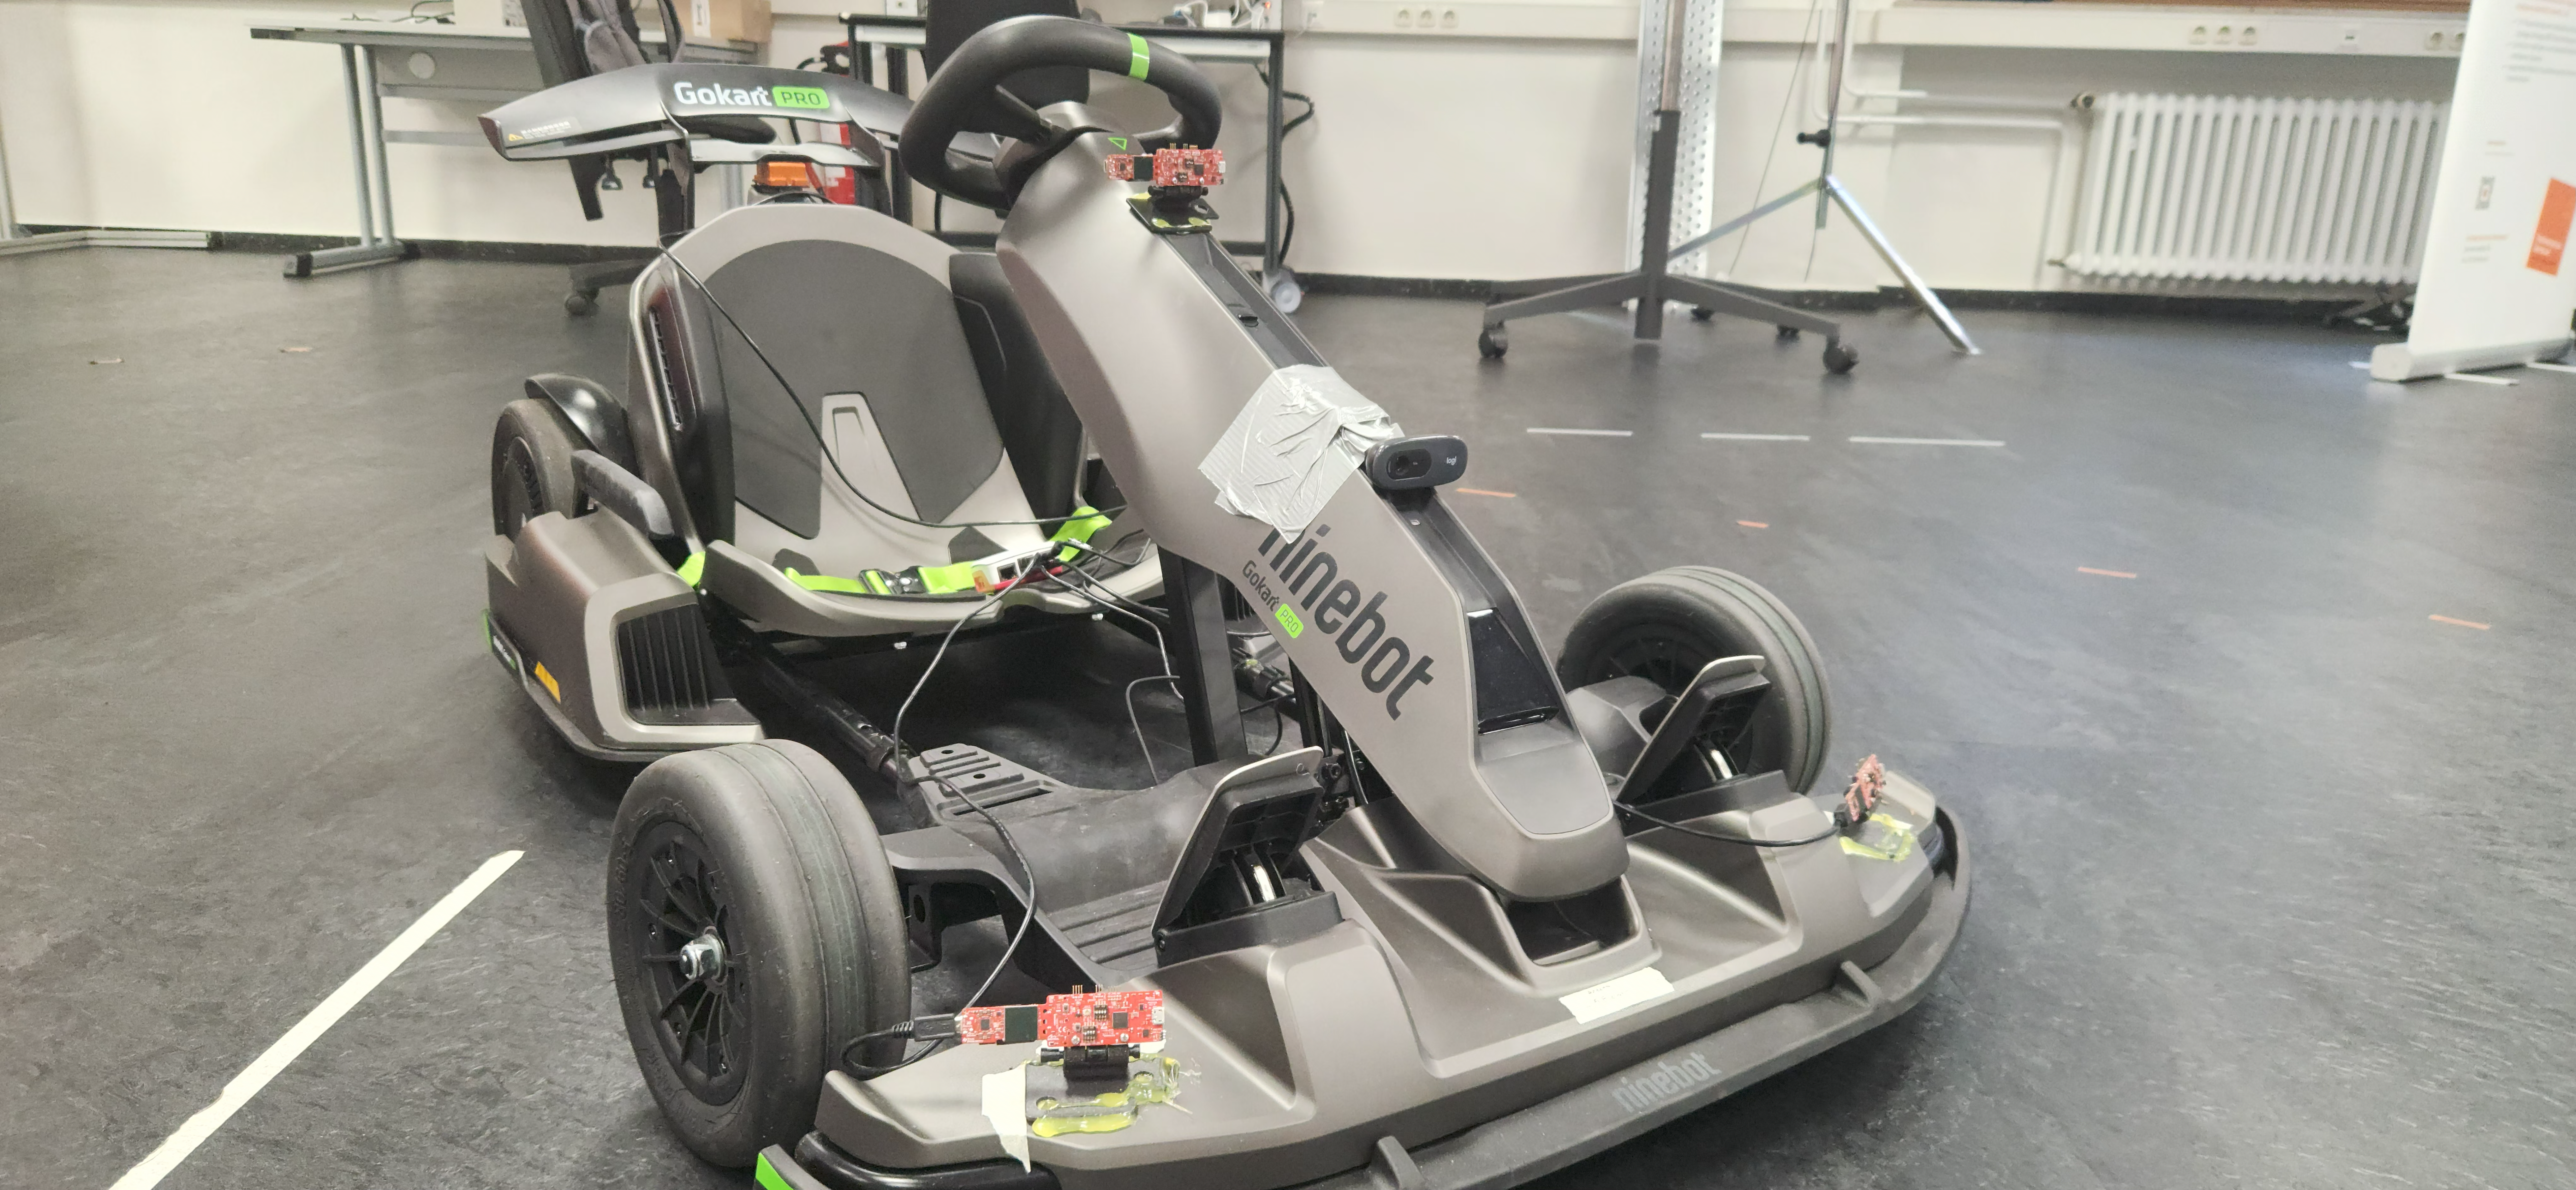
\includegraphics[width=0.9\linewidth]{images/vehicleSystem.png}
    \caption{Ninebot test-vehicle system.}
    \label{fig:Ninebot_system}
\end{figure}

\newpage
The contributions of this work can be summarized as follows:  
\begin{enumerate}
    \item A radar ego-motion pipeline using mmWave sensors for displacement measurements and an IMU for rotation, minimizing hardware cost and system complexity.
    \item Integration of Doppler velocity and RANSAC filtering to improve the separation of static and dynamic objects.
    \item Submap aggregation to mitigate point cloud sparsity and improve alignment stability.
    \item Object tracking via clusters to identify and filter dynamic objects from the ego-motion estimation.
    \item Experimental validation using real-world data collected from a vehicle-mounted mmWave radar system.  
\end{enumerate}
